%% Copernicus Publications Manuscript Preparation Template for LaTeX Submissions
%% ---------------------------------
%% This template should be used for copernicus.cls
%% The class file and some style files are bundled in the Copernicus Latex Package, which can be downloaded from the different journal webpages.
%% For further assistance please contact Copernicus Publications at: production@copernicus.org
%% https://publications.copernicus.org/for_authors/manuscript_preparation.html


%% Please use the following documentclass and journal abbreviations for discussion papers and final revised papers.

%% 2-column papers and discussion papers
\documentclass[essd, manuscript]{copernicus}

%% \usepackage commands included in the copernicus.cls:
%\usepackage[german, english]{babel}
%\usepackage{tabularx}
%\usepackage{cancel}
%\usepackage{multirow}
%\usepackage{supertabular}
%\usepackage{algorithmic}
%\usepackage{algorithm}
%\usepackage{amsthm}
%\usepackage{float}
%\usepackage{subfig}
%\usepackage{rotating}


\begin{document}

\title{TEXT}


% \Author[affil]{given_name}{surname}

\Author[]{}{}
\Author[]{}{}
\Author[]{}{}

\affil[]{ADDRESS}
\affil[]{ADDRESS}

%% The [] brackets identify the author with the corresponding affiliation. 1, 2, 3, etc. should be inserted.

%% If an author is deceased, please add a further affiliation and mark the respective author name(s) with a dagger, e.g. "\Author[2,$\dag$]{Anton}{Aman}" with the affiliations "\affil[2]{University of ...}" and "\affil[$\dag$]{deceased, 1 July 2019}"


\correspondence{NAME (EMAIL)}

\runningtitle{TEXT}

\runningauthor{TEXT}

\received{}
\pubdiscuss{} %% only important for two-stage journals
\revised{}
\accepted{}
\published{}

%% These dates will be inserted by Copernicus Publications during the typesetting process.

\firstpage{1}

\maketitle

\begin{abstract}
TEXT
\end{abstract}

\copyrightstatement{TEXT}

\introduction  %% \introduction[modified heading if necessary]

Changes in reflectance values or local textures that are separable from changes caused by other factors such as differences in atmospheric conditions, illumination and viewing angles, and soil moistures \citep{deng2008pca}.

The natural processes Earth surface 
The dynamics of the Earth surface follow defining a lower dimensional space.  he temporal variability of can be described using a number of components that is much lower than the images in the time series. From an algebra point of view, if each image is represented as a column of a matrix, we can say that this matrix has low rank. This fact has been already explored in remote sensing applying Principal Component Analysis (PCA) to compress and filter noise from images \citep{}.

PCA decomposes a matrix into its principal components or eigenvectors and eigenvalues presenting them in decreasing order of identif the eigenvectors of 
For the case of remote sensing images, the PCA decomposition of series of images captured through time typically shows a decrease in the eigenvalues in which the largest part of the original variance can be explained with only a few components. This fact has been used to compress and also filter out noise in the images coming from clouds and other atmospheric effects.

When applying PCA to remote sensing images it is required to filter out the noise in the images, which are typically contaminated with clouds and other atmospheric effects. If noise is not removed, most of the variability in the images will be and PCA will capture it in its components. One of the main drawbacks of applying PCA is its inability to work with missing values. Some alternative implementations of Singular Value Decomposition that can work with missing data have been proposed but it is a common practice to assign these values a fixed value or apply interpolation techniques to the data previous to calculating its PCA.

In this work we explore an alternative methodology to PCA based on neural networks that can work with missing values. This methodology is tested using Sentinel 2 data and its results are compared to PCA using interpolated data for the missing values. 

PCA using interpolated data. Cloud detection 


\section{Methodology}


There are many different possibilities of arranging the data before performing PCA or decomposing. 


\section{Data}

The Copernicus Sentinel-2 mission \citep{drusch2012sentinel} is a constellation of two polar-orbiting satellites Sentinel-2A and Sentinel-2B launched on the 23th of June 2015 and the 7th of March 2017, respectively. These satellites are placed in the same sun-synchronous orbit and scan the Earth with a combined revisit period of 5 days and spatial resolutions that range between 10 and 60 metres. Digital Earth Australia (DEA) \citep{dhu2017digital} is a platform that contains Sentinel-2 data for Australia. DEA facilitates access and enhances quality of the data by adding further processing, such as correction for atmospheric and terrain effects. DEA data is stored using the Albers equal area projection for ensuring pixel size remains constant independent of its location.

To run the experiments in this work we extracted from DEA a 7000 km\textsuperscript{2} area around the Australian Capital Territory region comprising the years 2018 and 2019. Spectrally, we chose a subset of seven bands: three in the visible channels, two in the near infra-red and two in the short wave infrared, corresponding to bands (2, 3, 4, 8, 8a, 11, 12) in the original dataset. Bands 8a, 11 and 12 have nominal resolutions of 20 metres and were upsampled into 10 metres using nearest neighbour, to achieve a homogeneous resolution across all bands.

The data was then split using regular tiles of 4 square kilometers each, comprising the whole temporal extent. Figure \ref{dataset} shows a map of the region and the extent of each tile within a 16 by 23 grid. Using a contiguous region, as opposed to sparse isolated tiles, ensures the dataset contains a fair mix of full and partial tiles due to tile boundaries. The objective is to consider a dataset that is maneageable to carry out the experiments but that is representative of the configuration variability of the original Sentinel-2 data. The results of this work should be easily reproduced for any other location.

\begin{figure}%
    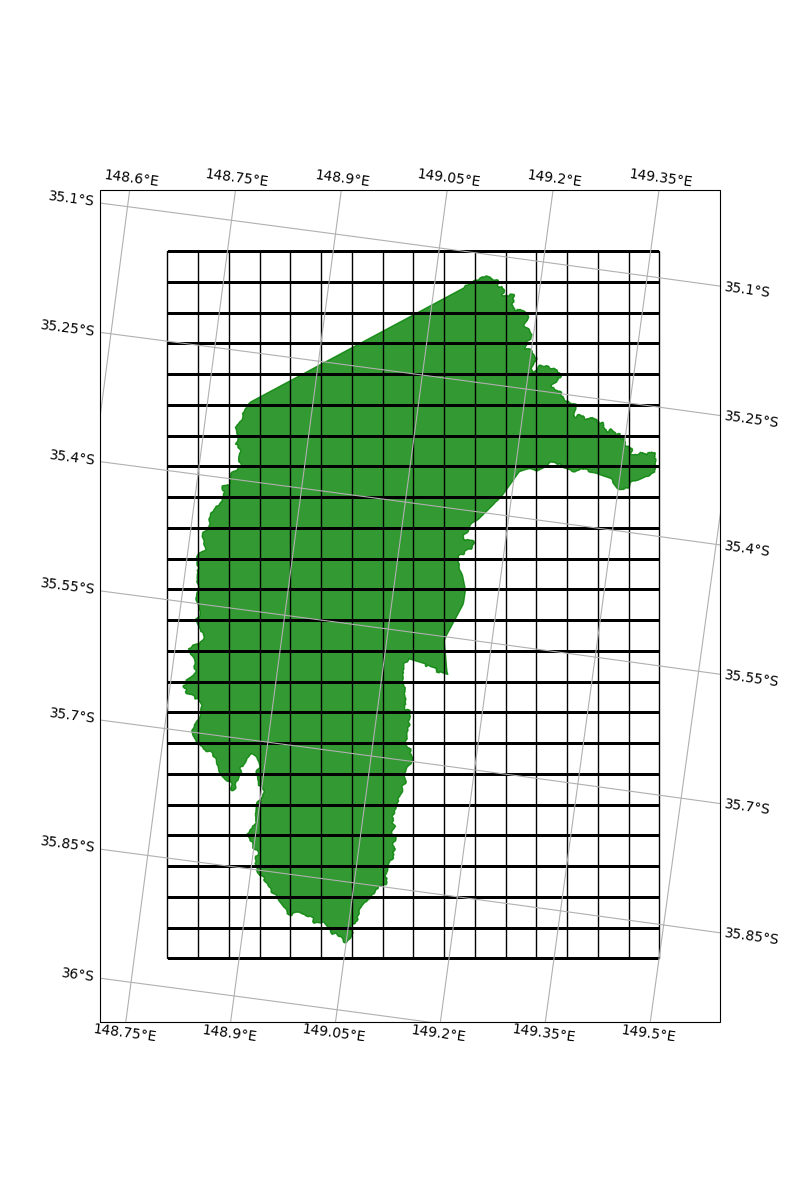
\includegraphics[width=14cm]{fig1.png}
    \caption{Region of the ACT with extents of the Sentinel 2 tiles.}%
    \label{dataset}%
\end{figure}

Each tile, as described previously, can be represented using a cube formed stacking 400 by 400 pixel images along the temporal dimension. In time, the number of images ranges between 85 and 130 depending on the position of the tile. The data was finally stored stacking each spectral band along the temporal dimension. Figure \ref{dataset_detail} represents the one of the tiles in the dataset, where images corresponding to different satellite acquisitions are stacked in the vertical dimension. On the left, the true colour composite is represented. On the right, the seven spectral bands are stacked together along the time dimension representing the final dataset used in the experiments. 

\begin{figure}%
    {{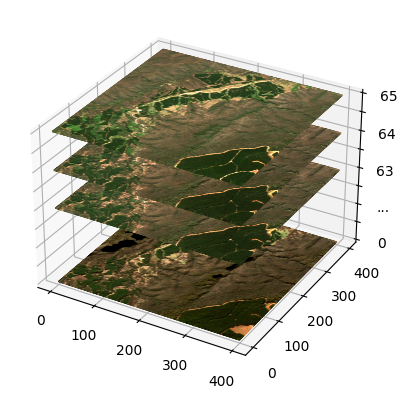
\includegraphics[width=8cm]{fig2a.png} }}%
    {{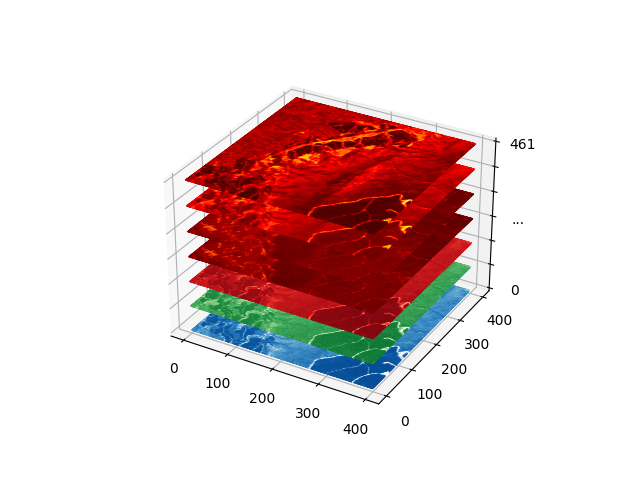
\includegraphics[width=8cm]{fig2b.png} }}%
    \caption{Tile corresponding to the top-left corner in the dataset (a) true colour representation, (b) multispectral stacked data}%
    \label{dataset_detail}%
\end{figure}


\subsection{Clouds and shadows filtering}
Remote sesing images are 


\section{Experimental Results and Discussion}
TEXT


\section{Conclusion}
In this paper, we evaluated the application of NNs to decompose remote sensing data in the presence of missing values. The methodology was evaluated to Sentinel-2 time series data for the Australian Capital Territory region. The NN-based methodology achieved better compression ratios and accuracy at interpolating missing values when compared to PCA. We demonstrate that relaxing the orthogonality constraints of PCA improves compression for time series of satellite multispectral data.

Additional studies are planned to evaluate the effect of non-linearities and convolution operations in the network. Another avenue for exploration is the introduction of constraints that lead to sparsity to enhance compression and improve interpretability of the results. 

TEXT

\conclusions  %% \conclusions[modified heading if necessary]
TEXT

%% The following commands are for the statements about the availability of data sets and/or software code corresponding to the manuscript.
%% It is strongly recommended to make use of these sections in case data sets and/or software code have been part of your research the article is based on.

\codeavailability{TEXT} %% use this section when having only software code available


\dataavailability{TEXT} %% use this section when having only data sets available


\codedataavailability{TEXT} %% use this section when having data sets and software code available


\sampleavailability{TEXT} %% use this section when having geoscientific samples available


\videosupplement{TEXT} %% use this section when having video supplements available


\appendix
\section{}    %% Appendix A

\subsection{}     %% Appendix A1, A2, etc.


\noappendix       %% use this to mark the end of the appendix section

%% Regarding figures and tables in appendices, the following two options are possible depending on your general handling of figures and tables in the manuscript environment:

%% Option 1: If you sorted all figures and tables into the sections of the text, please also sort the appendix figures and appendix tables into the respective appendix sections.
%% They will be correctly named automatically.

%% Option 2: If you put all figures after the reference list, please insert appendix tables and figures after the normal tables and figures.
%% To rename them correctly to A1, A2, etc., please add the following commands in front of them:

\appendixfigures  %% needs to be added in front of appendix figures

\appendixtables   %% needs to be added in front of appendix tables

%% Please add \clearpage between each table and/or figure. Further guidelines on figures and tables can be found below.



\authorcontribution{TEXT} %% this section is mandatory

\competinginterests{TEXT} %% this section is mandatory even if you declare that no competing interests are present

\disclaimer{TEXT} %% optional section

\begin{acknowledgements}
TEXT
\end{acknowledgements}




%% REFERENCES

%% The reference list is compiled as follows:

%%\begin{thebibliography}{}

%%\bibitem[AUTHOR(YEAR)]{LABEL1}
%%REFERENCE 1

%%\bibitem[AUTHOR(YEAR)]{LABEL2}
%%REFERENCE 2

%%\end{thebibliography}

%% Since the Copernicus LaTeX package includes the BibTeX style file copernicus.bst,
%% authors experienced with BibTeX only have to include the following two lines:
%%
\bibliographystyle{copernicus}
\bibliography{refs.bib}
%%
%% URLs and DOIs can be entered in your BibTeX file as:
%%
%% URL = {http://www.xyz.org/~jones/idx_g.htm}
%% DOI = {10.5194/xyz}


%% LITERATURE CITATIONS
%%
%% command                        & example result
%% \citet{jones90}|               & Jones et al. (1990)
%% \citep{jones90}|               & (Jones et al., 1990)
%% \citep{jones90,jones93}|       & (Jones et al., 1990, 1993)
%% \citep[p.~32]{jones90}|        & (Jones et al., 1990, p.~32)
%% \citep[e.g.,][]{jones90}|      & (e.g., Jones et al., 1990)
%% \citep[e.g.,][p.~32]{jones90}| & (e.g., Jones et al., 1990, p.~32)
%% \citeauthor{jones90}|          & Jones et al.
%% \citeyear{jones90}|            & 1990



%% FIGURES

%% When figures and tables are placed at the end of the MS (article in one-column style), please add \clearpage
%% between bibliography and first table and/or figure as well as between each table and/or figure.


%% ONE-COLUMN FIGURES

%%f
%\begin{figure}[t]
%\includegraphics[width=8.3cm]{FILE NAME}
%\caption{TEXT}
%\end{figure}
%
%%% TWO-COLUMN FIGURES
%
%%f
%\begin{figure*}[t]
%\includegraphics[width=12cm]{FILE NAME}
%\caption{TEXT}
%\end{figure*}
%
%
%%% TABLES
%%%
%%% The different columns must be seperated with a & command and should
%%% end with \\ to identify the column brake.
%
%%% ONE-COLUMN TABLE
%
%%t
%\begin{table}[t]
%\caption{TEXT}
%\begin{tabular}{column = lcr}
%\tophline
%
%\middlehline
%
%\bottomhline
%\end{tabular}
%\belowtable{} % Table Footnotes
%\end{table}
%
%%% TWO-COLUMN TABLE
%
%%t
%\begin{table*}[t]
%\caption{TEXT}
%\begin{tabular}{column = lcr}
%\tophline
%
%\middlehline
%
%\bottomhline
%\end{tabular}
%\belowtable{} % Table Footnotes
%\end{table*}
%
%%% LANDSCAPE TABLE
%
%%t
%\begin{sidewaystable*}[t]
%\caption{TEXT}
%\begin{tabular}{column = lcr}
%\tophline
%
%\middlehline
%
%\bottomhline
%\end{tabular}
%\belowtable{} % Table Footnotes
%\end{sidewaystable*}
%
%
%%% MATHEMATICAL EXPRESSIONS
%
%%% All papers typeset by Copernicus Publications follow the math typesetting regulations
%%% given by the IUPAC Green Book (IUPAC: Quantities, Units and Symbols in Physical Chemistry,
%%% 2nd Edn., Blackwell Science, available at: http://old.iupac.org/publications/books/gbook/green_book_2ed.pdf, 1993).
%%%
%%% Physical quantities/variables are typeset in italic font (t for time, T for Temperature)
%%% Indices which are not defined are typeset in italic font (x, y, z, a, b, c)
%%% Items/objects which are defined are typeset in roman font (Car A, Car B)
%%% Descriptions/specifications which are defined by itself are typeset in roman font (abs, rel, ref, tot, net, ice)
%%% Abbreviations from 2 letters are typeset in roman font (RH, LAI)
%%% Vectors are identified in bold italic font using \vec{x}
%%% Matrices are identified in bold roman font
%%% Multiplication signs are typeset using the LaTeX commands \times (for vector products, grids, and exponential notations) or \cdot
%%% The character * should not be applied as mutliplication sign
%
%
%%% EQUATIONS
%
%%% Single-row equation
%
%\begin{equation}
%
%\end{equation}
%
%%% Multiline equation
%
%\begin{align}
%& 3 + 5 = 8\\
%& 3 + 5 = 8\\
%& 3 + 5 = 8
%\end{align}
%
%
%%% MATRICES
%
%\begin{matrix}
%x & y & z\\
%x & y & z\\
%x & y & z\\
%\end{matrix}
%
%
%%% ALGORITHM
%
%\begin{algorithm}
%\caption{...}
%\label{a1}
%\begin{algorithmic}
%...
%\end{algorithmic}
%\end{algorithm}
%
%
%%% CHEMICAL FORMULAS AND REACTIONS
%
%%% For formulas embedded in the text, please use \chem{}
%
%%% The reaction environment creates labels including the letter R, i.e. (R1), (R2), etc.
%
%\begin{reaction}
%%% \rightarrow should be used for normal (one-way) chemical reactions
%%% \rightleftharpoons should be used for equilibria
%%% \leftrightarrow should be used for resonance structures
%\end{reaction}
%
%
%%% PHYSICAL UNITS
%%%
%%% Please use \unit{} and apply the exponential notation


\end{document}
